\chapter{Temporal Logic of Actions}

\section{Introduction}

% TLA Plus origins and Uses 

% TLA Tools

% TLA learning resources
\begin{itemize}
    \item \href{https://lamport.azurewebsites.net/tla/summary-standalone.pdf}{A summary of TLA}
    \item 
\end{itemize}


\unfinished

\section{Terminology}
\begin{definitionbox}{Stuttering Step}
    A transition where all state variables stay the same. Represented in TLA+ using the actions:
    \[\begin{matrix*}[l]
        [A]_v & \text{Action }A \text{ occurs, or }v \text{ is unchanged in successor} \\
        [A]_{\langle v_1,v_2,v_3\rangle} & \text{Same as above but with many variables} \\
    \end{matrix*}\]
\end{definitionbox}
\begin{definitionbox}{Actions}
    Change the state of a module (primed variables $\to$ non-primed)
\end{definitionbox}
\subsection{TLA+ Constructs}
Based on an excellent cheat sheet created by professor Narankar Dulay, based on \href{https://mbt.informal.systems/docs/tla_basics_tutorials/tla+cheatsheet.html}{Model Based Testing \@ Informal Systems's own}.

\subsubsection{File Structure}
\begin{minipage}{.48\textwidth}
    \tlatex
\@x{}\moduleLeftDash\@xx{ {\MODULE} name}\moduleRightDash\@xx{}%
\@x{ {\EXTENDS} m1 ,\, \.{\dots} ,\, mN\@s{8.2}}%
\@y{\@s{0}%
 extends multiple modules
}%
\@xx{}%
\@x{ {\CONSTANTS} c1 ,\, \.{\dots} ,\, cN\@s{4.73}}%
\@y{\@s{0}%
 constants are defined in the \ensuremath{.cfg} file
}%
\@xx{}%
\@x{ {\VARIABLES} v1 ,\, \.{\dots} ,\, vN}%
\@x{ Vars\@s{0.29} \.{\defeq} {\langle} v1 ,\, \.{\dots} ,\, vN {\rangle}}%
\@x{ Type \.{\defeq} v1\_formula \.{\land} \.{\dots} \.{\land} vN\_formula}%
\@x{}\midbar\@xx{}%
\@x{}%
\@y{\@s{0}%
 Specification for state machine
}%
\@xx{}%
\@pvspace{8.0pt}%
\@x{ Init\@s{5.52} \.{\defeq} formula}%
\@y{\@s{0}%
 Initial state
}%
\@xx{}%
\@x{ Def1 \.{\defeq} formula}%
\@y{\@s{0}%
 Definitions (any number of)
}%
\@xx{}%
\@pvspace{8.0pt}%
\@x{}%
\@y{\@s{0}%
 Can have any number of subactions of \ensuremath{Next
}}%
\@xx{}%
\@x{ Action1 \.{\defeq} action\_formula}%
\@pvspace{8.0pt}%
\@x{}%
\@y{\@s{0}%
 Determine \ensuremath{Next} State
}%
\@xx{}%
\@x{ Next \.{\defeq} Action1 \.{\lor} \.{\dots} \.{\lor} ActionN}%
\@x{}\midbar\@xx{}%
\@x{ Fair\@s{0.24} \.{\defeq} fairness\_formula \.{\land} \.{\dots}}%
\@x{ Spec \.{\defeq} Init \.{\land} {\Box} [ Next ]_{ Vars} \.{\land} Fair}%
\@x{}\midbar\@xx{}%
\@x{ NotDeadlock \.{\defeq} {\Box} ( {\ENABLED} Next )}%
\@y{\@s{0}%
 Properties
}%
\@xx{}%
\@x{ Typed \.{=} {\Box} Type}%
\@x{}\bottombar\@xx{}%

\end{minipage}
\hfill
\begin{minipage}{.48\textwidth}
    \inputminted{text}{tla_plus/code/ExampleFile.tla}
\end{minipage}
\vspace{.3cm}

\newcommand{\TLAset}[1]{\textcolor{blue}{\mintinline{text}{#1}}}
\newcommand{\TLAbool}[1]{\textcolor{red}{\mintinline{text}{#1}}}
\newcommand{\TLAinteger}[1]{\textcolor{orange}{\mintinline{text}{#1}}}
\newcommand{\TLAfunction}[1]{\textcolor{ForestGreen}{\mintinline{text}{#1}}}
\newcommand{\TLAtuple}[1]{\textcolor{purple}{\mintinline{text}{#1}}}
\newcommand{\TLAother}[1]{\textcolor{black}{\mintinline{text}{#1}}}

For the language definitions, the following key is used:
\\ \centerline{\TLAbool{Booleans} \ \TLAfunction{Functions} \ \TLAinteger{Integers} \ \TLAset{Sets} \ \TLAtuple{Tuples \& Sequences}}

\subsubsection{Logic}
    \begin{tabular}{l l p{.8\textwidth}}
        \BOOLEAN & \TLAset{BOOLEAN} & Set of boolean values $\{true, false\}$ \\
        \TRUE & \TLAbool{TRUE} \\
        \FALSE & \TLAbool{FALSE} \\
        $\lnot$ & \TLAbool{~e} & Logical negation \\
        $a \land b$ & \TLAbool{a /\ b} & Logical and \\
        $a \lor b$ & \TLAbool{a \/ b} & Logical or \\
        $a = b$ & \TLAbool{a = b} & Equality \\
        $a \neq b$ & \textcolor{red}{a \# b} & Not equal \\
        $a \implies b$ & \TLAbool{a => b} & Logical Implication ($b \lor \neg a$) or \TLAbool{IF a THEN b ELSE TRUE}\\
        $a \equiv b$ & \TLAbool{a <=> b} & Equivalence \\
    \end{tabular}

\subsubsection{Quantifiers}

    \begin{tabular}{l l p{.6\textwidth}}
        $\A\, var \.{\in} S \.{:} e$ & \TLAbool{\A var \in S: e} & Expression $e$ is $true$ for all elements of set $S$\\
        $\E\, var \.{\in} S \.{:} e$ & \TLAbool{\E var \in S: e} & Expression $e$ is $true$ for some element of set $S$\\
        ${\CHOOSE} var \.{\in} S \.{:} e$ & \TLAother{CHOOSE var \in S : e} & Always picks the same element $e$ from set $S$ (undefined for empty sets) \\
    \end{tabular}

\subsubsection{Integers}

    \begin{tabular}{l l p{.7\textwidth}}
        $Int$ & \TLAset{Int} & Set of all integers \\
        $Nat$ & \TLAset{Nat} & Set of all natural numbers (not including $0$) \\
        $1, -2, 12542355$ & \TLAinteger{1, -2, 12542355} & Integer literals \\
        $a \dotdot b$ & \TLAset{a..b} & Integer range as a set (inclusive and empty is $a > b$) \\
        $a + b, a - b, a * b$ & \TLAinteger{a + b, a - b, a * b} & \multirow{2}{*}{Integer arithmetic} \\
        $a ^ b, a \% b$ & \TLAinteger{a ^ b, a \% b} & \\
        $a > b, a \geq b, a < b, a \leq b$ & \TLAbool{a > b, a >= b, a < b, a <= b} & Comparison operations \\
    \end{tabular}


\subsubsection{Strings}

    \begin{tabular}{l l p{.7\textwidth}}
        $\STRING$ & \TLAset{STRING} & The set of all finite strings \\
        "", "hello world" & \TLAset{"", "hello world"} & String literals \\
    \end{tabular}


\subsubsection{Finite Sets}


    \begin{tabular}{l l p{.7\textwidth}}
        $\{ a ,\, b ,\, c \}$ & \TLAtuple{{a,b,c}} & A set constructed of $a,b$ and $c$ (al the same type) \\
        $Cardinality ( S )$ & \TLAinteger{Cardinality(S)} & Get the size/cardinality of set $S$ \\
        $e \in S, e \notin S$ & \TLAbool{e \in S, e \notin S} & Checking set membership \\
        $S1 \subseteq S2$ & \TLAbool{S1 \subseteq S2} & Checking a $S1$ is a subset (can be equal) \\
        $S1 \cup S2$ & \TLAset{S1 \union S2} or \TLAset{S1 \cup S2} & Set union operation \\
        $S1 \cap S2$ & \TLAset{S1 \intersection S2} or \TLAset{S1 \cap S2} & Set intersection \\
        $S1 \backslash S2$ & \TLAset{S1 \ S2} & Set difference ($S1 - S2$) \\
        $\{var k \in S: P(var)\}$ & \TLAset{{var \in S: P(m)}} & Filter elements of $S$ using predicate $P$ \\ 
        $\{e: k \in KeyS\}$ & \TLAfunction{{e: k \in KeyS}} & Map all keys from $Keys$ with expression $e$ \\
    \end{tabular}


\subsubsection{Functions \& Maps}

    \begin{tabular}{l l p{.5\textwidth}}
        $k \in keys \mapsto e$ & \TLAfunction{[k \in KeyS |-> e]} & [Function Construction] map all keys $k$ to expression $e$ (which potentially uses $k$) \\
        $fn[k]$ & \TLAother{fn[k]} & [Function Application] get value associated to key $k$ by function $fn$ \\
        $[ fn {\EXCEPT} \bang [ k1 ] = e1, \dots ]$ & \TLAfunction{[fn EXCEPT ![k1] = e1, ...} & Remap the key $k1$ for function $fn$ (can use \TLAother{@} to reference the original $fn[k1]$) with other remapings (the $\dots$) \\
        $[Keys \rightarrow Values]$ & \TLAset{Keys -> Values} & The set of all functions mapping the set of $Keys$ to the set of $Values$, (e.g $STRING \rightarrow Nat$) \\
    \end{tabular}


\subsubsection{Records}

    \begin{tabular}{l l p{.4\textwidth}}
        $[f1 \mapsto e1, f2 \mapsto e2, \dots]$ & \TLAfunction{[f1 |-> e1, f2 |-> e2, ...]} & Construct a record of fields $f$s containing expressions $e$s \\
        $myRec.f$ & \TLAother{myRec.f} & Access field $f$ from a record $myRec$ \\
        $[myRec \EXCEPT \bang . f1 = e1, \dots]$ & \TLAfunction{[rec EXCEPT !.f1 = e1, ...]} & Rebinding fields (similar to rebinding keys for functions) \\
        $[f1: S1, f2: S2, \dots]$ & \TLAset{[f1: S1, f2: S2, ...]} & The set of all records with field names $f$s in sets $S$s \\
    \end{tabular}


\subsubsection{Sequences}

    \begin{tabular}{l l p{.5\textwidth}}
        $\langle e1, e2, e3 \rangle$ & \TLAtuple{<<e1, e2, e3>>} & Construct a sequence (list) from expressions (all the same type) \\
        $mySeq[i]$ & \TLAother{mySeq[i]} & Get index $i$ of sequence $mySeq$ (indexed from 1) \\
        $seq1 \circ seq2$ & \TLAtuple{seq1 \o seq2} & Concatenation of sequences \\
        $Len(mySeq)$ & \TLAinteger{Len(mySeq)} & Length of a given sequence \\
        $Append(mySeq, e)$ & \TLAtuple{Append(mySeq, e)} & Add to end of a sequence \\
        $Head(mySeq)$ & \TLAother{head(mySeq)} & Get first element of $mySeq$ \\
        $Seq(S)$ & \TLAset{Seq(S)} & The set of all finite sequences over set $S$ \\
    \end{tabular}


\subsubsection{Tuples}

    \begin{tabular}{l l p{.5\textwidth}}
        $\langle a, b, c \rangle$ & \TLAtuple{<<a, b, c>>} & Construct a tuple (types of elements can be different) \\
        $myTup[i]$ & \TLAother{myTup[i]} & Index a tuple \\
        $S1 \times S2 \times ... \times Sn$ & \TLAset{S1 \X S2 \X ... \X Sn} & Set of the cartesian product of the sets of tuples (each tuple of form $\langle s1, s2, \dots sn\rangle$) \\
    \end{tabular}


\subsubsection{Miscellanous}

    \begin{tabular}{l l p{.5\textwidth}}
        $\LET var \defeq e1 \in e2$ & \TLAother{LET var == e1 \in e2} & A let statement (e.g same as in Haskell) \\
        $\IF e \THEN e1 \ELSE e2$ & \TLAother{IF e THEn e1 ELSE e2} & If statements (statement is an expression itself - e.g like Elixir, Haskell, Rust) \\
    \end{tabular}


\subsubsection{Actions}

    \begin{tabular}{l l p{.5\textwidth}}
        $var'$ & \TLAother{var'} & [Primed variable] denotes the non-primed $var$ in the next state \\
        $\UNCHANGED \langle v1, v2, \dots\rangle$ & \TLAset{UNCHANGED <<v1, v2, ...>>} & Shorthand for $v1 = v1' \land v2 = v2' \land \dots$ \\
        $[A]_v, [A]_{\langle v1, v2, \dots\rangle}$ & \TLAset{[A]_v, [A]_<<v1, v2, ... >>} & Stuttering action (can apply action or variables $v$, $v1, v2, \dots$ are unchanged) \\
        $\langle A \rangle_v , \langle A \rangle_{\langle v1, v2, \dots \rangle}$ & \TLAset{<<A>>_v, <A>_<<v1,v2,v3>>} & Non-stuttering acton, the variables must $v$, $v1, v2, \dots$ change \\
        $\ENABLED A$ & \TLAset{ENABLED A} & $true$ if action $A$ is enabled \\
    \end{tabular}


\subsubsection{Temporal Logic}

    \begin{tabular}{l l p{.5\textwidth}}
        $\Box F$ & \TLAset{[]F} & F is always $true$ \\
        $\Diamond F$ & \TLAset{<>F} & F is eventually $true$ \\
        $F1 \leadsto F2$ & \TLAset{F1 ~> F2} & $F1$ leads to $F2$ \\
        $WF_v(A), SF_v(A)$ & \TLAset{WF_v(A), SF_v(A)} & Strong and weak fairness for action $A$ \\ 
    \end{tabular}

\section{Examples}
\subsection{One Bit Clock}
\begin{minipage}{.48\textwidth}
    \tlatex
\@x{}\moduleLeftDash\@xx{ {\MODULE} OneBitClock}\moduleRightDash\@xx{}%
\@x{ {\VARIABLE} b}%
\@x{ Type \.{\defeq} b \.{\in} \{ 0 ,\, 1 \}}%
\@x{}\midbar\@xx{}%
\@x{ Init\@s{4.12} \.{\defeq} b \.{=} 0 \.{\lor} b \.{=} 1}%
 \@x{ Next \.{\defeq} ( ( b \.{=} 0 ) \.{\land} ( b \.{'} \.{=} 1 ) ) \.{\lor}
 ( ( b \.{=} 1 ) \.{\land} ( b \.{'} \.{=} 0 ) )}%
\@x{ Spec\@s{1.46} \.{\defeq} Init \.{\land} {\Box} [ Next ]_{ b}}%
\@x{}\midbar\@xx{}%
\@x{ Typed \.{\defeq} {\Box} Type}%
\@x{}\bottombar\@xx{}%

\end{minipage}
\hfill
\begin{minipage}{.48\textwidth}
    \inputminted{text}{tla_plus/code/OneBitClock.tla}
\end{minipage}
\vspace{.3cm}
\\ A basic counter with states $\dots \to 0 \to 1 \to 0 \to 1 \to \dots$.
\begin{itemize}
    \item Contains a single variable $b$ ($b'$ is the value of $b$ in the next state).
    \item Starts as $0$ or $1$, and is always $0$ or $1$ (by the theorem $Typed$ which states $Type$ is always true)
    \item $b$ is always updated in the next 
\end{itemize}
The use of $Init \land \Box[Next]_b$ is equivalent to $Init \land \Box(Next \lor (b = b'))$ and allows for a \textit{stuttering step}.

\subsection{12 Hour Clock}
\begin{minipage}{.48\textwidth}
    \tlatex
\@x{}\moduleLeftDash\@xx{ {\MODULE} TwelveHourClock}\moduleRightDash\@xx{}%
\@x{ {\EXTENDS} Naturals}%
\@x{ {\VARIABLE} hour}%
\@x{}\midbar\@xx{}%
\@x{ Init\@s{4.12} \.{\defeq} hour \.{\in} 0 \.{\dotdot} 11}%
\@x{ Next \.{\defeq} hour \.{'} \.{=} ( hour \.{+} 1 ) \.{\%} 12}%
\@x{ Spec\@s{1.46} \.{\defeq} Init \.{\land} {\Box} [ Next ]_{ hour}}%
\@x{}\midbar\@xx{}%
\@x{ Typed \.{\defeq} {\Box} Init}%
\@x{}\bottombar\@xx{}%

\end{minipage}
\hfill
\begin{minipage}{.48\textwidth}
    \inputminted{text}{tla_plus/code/TwelveHourClock.tla}
\end{minipage}
\vspace{.3cm}
\\ The $Init$ predicate is always true (from $Typed \triangleq \Box Init$) hence TLC can check the correctness of our $Next$ implementation.

\subsection{24 Hour Clock}
We can make use of TLC provided functions such as $Print$ and $PrintT$.
\\
\tlatex
\@x{}\moduleLeftDash\@xx{ {\MODULE} 24HourClock}\moduleRightDash\@xx{}%
\@x{ {\EXTENDS} Naturals ,\, TLC}%
\@x{ {\VARIABLE} hour}%
\@x{}\midbar\@xx{}%
\@x{ Init\@s{4.12} \.{\defeq} hour \.{\in} 0 \.{\dotdot} 23}%
\@x{ Next \.{\defeq} hour \.{'} \.{=} ( hour \.{+} 1 ) \.{\%} 24}%
\@x{\@s{39.83} \.{\land} (}%
 \@x{\@s{55.04} ( hour \.{\leq} 12 \.{\land} PrintT ( {\langle}\@w{[Morning]\
 time:} ,\, hour {\rangle} ) )}%
 \@x{\@s{43.93} \.{\lor} ( hour \.{>} 12 \.{\land} hour \.{<} 18 \.{\land}
 PrintT ( {\langle}\@w{[Afternoon]\ time:} ,\, hour {\rangle} ) )}%
 \@x{\@s{43.93} \.{\lor} ( hour \.{\geq} 18 \.{\land} PrintT (
 {\langle}\@w{[Evening]\ time:} ,\, hour {\rangle} ) )}%
\@x{\@s{39.83} )}%
 \@x{ Spec\@s{1.46} \.{\defeq} Init \.{\land} {\langle} Next {\rangle}_{
 hour}}%
\@x{}\midbar\@xx{}%
\@x{ Typed \.{\defeq} {\Box} Init}%
\@x{}\bottombar\@xx{}%

\inputminted{text}{tla_plus/code/24HourClock.tla}
We can see the short-circuiting of $\lor$ resulting in messages being printed, $PrintT$ always returns $true$:
\\
\\ \begin{minipage}{.33\textwidth}
\begin{minted}{bash}
<<"[Morning] time:", 0>>
<<"[Morning] time:", 1>>
<<"[Morning] time:", 2>>
<<"[Morning] time:", 3>>
<<"[Morning] time:", 4>>
<<"[Morning] time:", 5>>
<<"[Morning] time:", 6>>
<<"[Morning] time:", 7>>
\end{minted}  
\end{minipage}
\begin{minipage}{.33\textwidth}
\begin{minted}{bash}
<<"[Morning] time:",   8>>
<<"[Morning] time:",   9>>
<<"[Morning] time:",   10>>
<<"[Morning] time:",   11>>
<<"[Morning] time:",   12>>
<<"[Afternoon] time:", 13>>
<<"[Afternoon] time:", 14>>
<<"[Afternoon] time:", 15>>
\end{minted}
\end{minipage}
\begin{minipage}{.33\textwidth}
\begin{minted}{bash}
<<"[Afternoon] time:", 16>>
<<"[Afternoon] time:", 17>>
<<"[Evening] time:",   18>>
<<"[Evening] time:",   19>>
<<"[Evening] time:",   20>>
<<"[Evening] time:",   21>>
<<"[Evening] time:",   22>>
<<"[Evening] time:",   23>>
\end{minted}
\end{minipage}

\section{Model Checking with TLC}
TLC uses a \mintinline{bash}{.cfg} file to configure the parameters for running the model checker.
\begin{minted}{text}
\* Defines a state machine 
SPECIFICATION Spec

\* Properties that must be true for every state
PROPERTY NotDeadlock Typed   \* Note TLC checks for absence of deadlock by default

\* Specifying invariants
INVARIANT Type   \* equivalent to PROPERTY []Type

\* Define constant values
CONSTANT Data = {1,2}

\* Specifying the init and next states
INIT Init
NEXT Next
\end{minted}
The TLC model checker performs a breadth-first search of all possible states to check properties hold, or the reachable state in which a violation takes place.
\begin{itemize}
    \item Safety properties can be encoded (if violated in any state at any time, property is violated)
    \item Liveness is encoded as determining that for times $\exists t' . \forall t. [satisified(state(t')) \land t' \geq t]$.
\end{itemize}

\subsection{Asynchronous Messages}
\begin{center}
    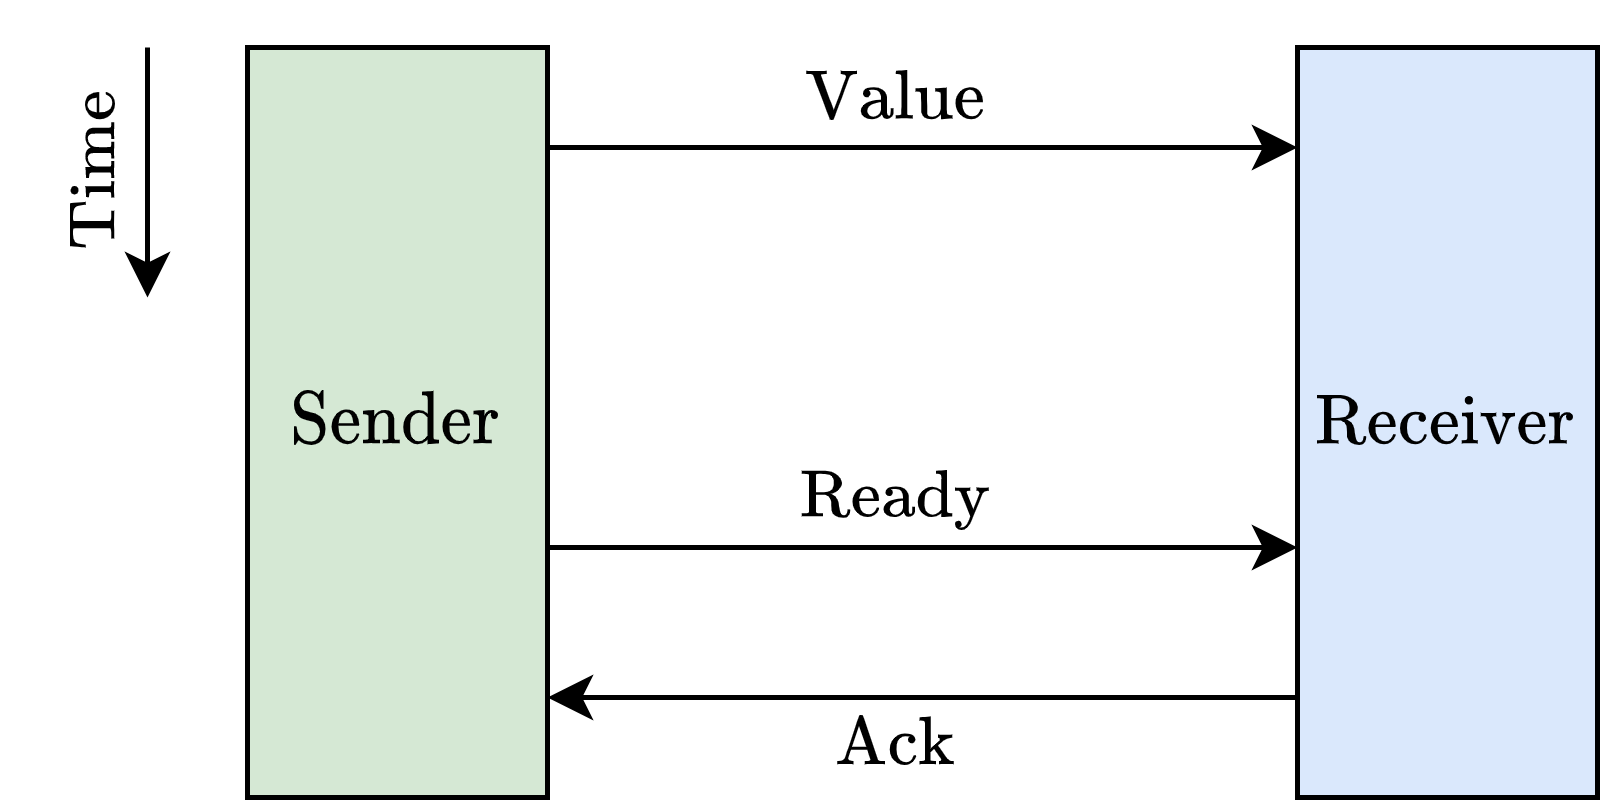
\includegraphics[width=.5\textwidth]{tla_plus/images/async_msg.drawio.png}
\end{center}
\subsubsection{TLA+}
\tlatex
\@x{}\moduleLeftDash\@xx{ {\MODULE} AsyncMessage}\moduleRightDash\@xx{}%
\@x{ {\EXTENDS} Naturals}%
\@x{ {\CONSTANT} Data}%
\@pvspace{8.0pt}%
\@x{ {\VARIABLES} value ,\, ready ,\, ack}%
\@x{ Vars\@s{0.29} \.{\defeq} {\langle} value ,\, ready ,\, ack {\rangle}}%
\@y{\@s{0}%
 Collection of variables values
}%
\@xx{}%
 \@x{ Type \.{\defeq} value \.{\in} Data \.{\land} ready \.{\in} \{ 0 ,\, 1 \}
 \.{\land} ack \.{\in} \{ 0 ,\, 1 \}}%
\@x{}\midbar\@xx{}%
\@pvspace{8.0pt}%
\@x{}%
\@y{\@s{0}%
 Initial state
}%
\@xx{}%
 \@x{ Init \.{\defeq} value \.{\in} Data \.{\land} ready \.{\in} \{ 0 ,\, 1 \}
 \.{\land} ack \.{=} ready}%
\@pvspace{8.0pt}%
\@x{}%
\@y{\@s{0}%
 Action to send a message (not yet acknowledged)
}%
\@xx{}%
 \@x{ Send \.{\defeq} ready \.{=} ack \.{\land} value \.{'} \.{\in} Data
 \.{\land} ready \.{'} \.{=} 1 \.{-} ready \.{\land} {\UNCHANGED} {\langle}
 ack {\rangle}}%
\@pvspace{8.0pt}%
\@x{}%
\@y{\@s{0}%
 Action to recieve a message with acknowledgement
}%
\@xx{}%
 \@x{ Receive \.{\defeq} ready \.{\neq} ack \.{\land} ack \.{'} \.{=} 1 \.{-}
 ack \.{\land} {\UNCHANGED} {\langle} value ,\, ready {\rangle}}%
\@pvspace{8.0pt}%
\@x{}%
\@y{\@s{0}%
 Module can either send or recieve (cannot do both due to unchanged in both
 actions)
}%
\@xx{}%
\@x{ Next \.{\defeq} Send \.{\lor} Receive}%
\@pvspace{8.0pt}%
\@x{}%
\@y{\@s{0}%
 \ensuremath{Init} is true, and next is always true with \ensuremath{Vars}
 potentially changed
}%
\@xx{}%
\@x{ Spec \.{\defeq} Init \.{\land} {\Box} [ Next ]_{ Vars}}%
\@x{}\midbar\@xx{}%
\@x{}%
\@y{\@s{0}%
 Constraints: Value is always in data, ready \& \ensuremath{ack} are always 0
 or 1
}%
\@xx{}%
\@x{ Typed \.{\defeq} {\Box} Type}%
\@x{}\bottombar\@xx{}%

\subsubsection{Code}
\inputminted{text}{tla_plus/code/AsyncMessage.tla}
\subsubsection{Configuration}
\inputminted{text}{tla_plus/code/AsyncMessage.cfg}

\subsection{Channel}
\begin{center}
    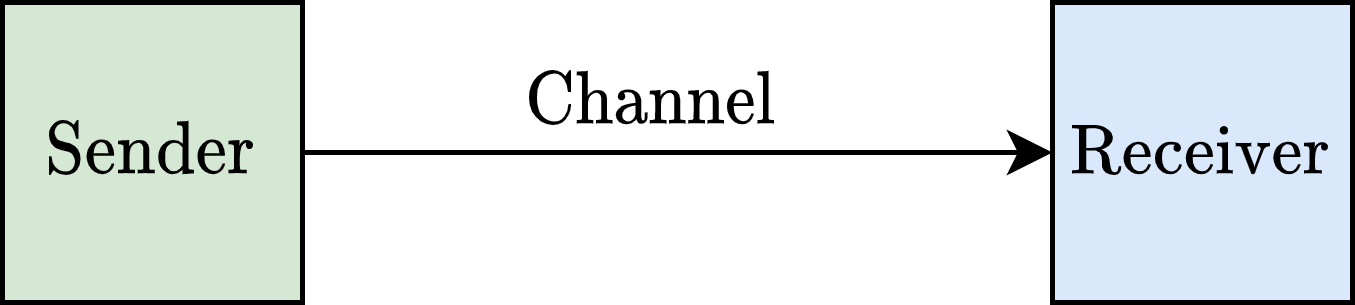
\includegraphics[width=.5\textwidth]{tla_plus/images/channel.drawio.png}
\end{center}
\subsubsection{TLA+}
\tlatex
\@x{}\moduleLeftDash\@xx{ {\MODULE} Channel}\moduleRightDash\@xx{}%
\@x{ {\EXTENDS} Naturals}%
\@x{ {\CONSTANT} Data}%
\@x{ {\VARIABLE} channel}%
\@pvspace{8.0pt}%
\@x{}%
\@y{\@s{0}%
 Check whether channel is in the set (created by use of
 \ensuremath{\.{\dotdot}}) of valid records
}%
\@xx{}%
 \@x{ Type \.{\defeq} channel \.{\in} [ value \.{:} Data ,\, ready \.{:} 0
 \.{\dotdot} 1 ,\, ack \.{:} 0 \.{\dotdot} 1 ]}%
\@pvspace{8.0pt}%
\@x{}\midbar\@xx{}%
\@x{ Init \.{\defeq} Type \.{\land} channel . ack \.{=} channel . ready}%
\@pvspace{8.0pt}%
\@x{}%
\@y{\@s{0}%
 Set value to \ensuremath{d} and flip ready
}%
\@xx{}%
 \@x{ Send ( d ) \.{\defeq} channel . ready \.{=} channel . ack \.{\land}
 channel \.{'} \.{=} [ channel {\EXCEPT} {\bang} . value \.{=} d ,\, {\bang}
 . ready \.{=} 1 \.{-} @ ]}%
\@pvspace{8.0pt}%
\@x{}%
\@y{\@s{0}%
 Flip \ensuremath{ack}, otherwise leave channel the same
}%
\@xx{}%
 \@x{ Receive \.{\defeq} channel . ready \.{\neq} channel . ack \.{\land}
 channel \.{'} \.{=} [ channel {\EXCEPT} {\bang} . ack \.{=} 1 \.{-} @ ]}%
\@pvspace{8.0pt}%
\@x{}%
\@y{\@s{0}%
 Can only send valuesa that are in \ensuremath{Data
}}%
\@xx{}%
\@x{ SendSome \.{\defeq} \E\, d \.{\in} Data \.{:} Send ( d )}%
\@pvspace{8.0pt}%
\@x{}%
\@y{\@s{0}%
 Either send or receieve (note can both send and recieve at the same time)
}%
\@xx{}%
\@x{ Next \.{\defeq} SendSome \.{\lor} Receive}%
\@pvspace{8.0pt}%
\@x{ Spec\@s{1.46} \.{\defeq} Init \.{\land} {\Box} [ Next ]_{ channel}}%
\@x{}\midbar\@xx{}%
\@x{ Typed \.{\defeq} {\Box} Type}%
\@x{}\bottombar\@xx{}%

\subsubsection{Code}
\inputminted{text}{tla_plus/code/Channel.tla}
\subsubsection{Configuration}
\inputminted{text}{tla_plus/code/Channel.cfg}

\subsection{Unbounded FIFO}
\begin{center}
    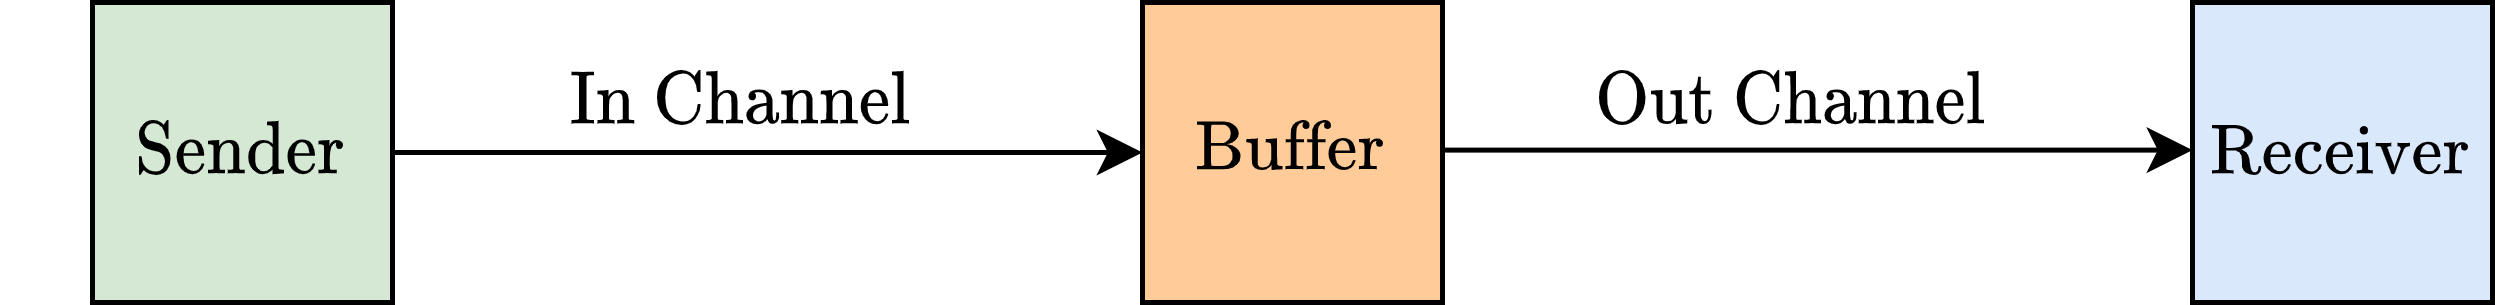
\includegraphics[width=.5\textwidth]{tla_plus/images/unbounded_FIFO.drawio.png}
\end{center}
\unfinished
